\documentclass[a4paper, 12pt]{article}

% packages
\usepackage{amssymb}
\usepackage[fleqn]{mathtools}
\usepackage{tikz}
\usepackage{enumerate}
\usepackage{bussproofs}
\usepackage{xcolor}
\usepackage[margin=1.3cm]{geometry}
\usepackage{logicproof}
\usepackage{diagbox}
\usepackage{listings}
\usepackage{graphicx}
\usepackage{lstautogobble}
\usepackage{hyperref}
\usepackage{multirow}
\usepackage{tipa}
\usepackage{pgfplots}

% tikz libraries
\usetikzlibrary{
    decorations.pathreplacing,
    arrows,
    shapes.gates.logic.US,
    circuits.logic.US,
    calc,
    automata,
    positioning,
    intersections
}

\pgfplotsset{compat=1.16}

\pgfmathdeclarefunction{gauss}{2}{%
  \pgfmathparse{1/(#2*sqrt(2*pi))*exp(-((x-#1)^2)/(2*#2^2))}%
}

\allowdisplaybreaks % allow environments to break
\setlength\parindent{0pt} % no indent

% shorthand for verbatim
% this clashes with logicproof, so maybe fix this at some point?
\catcode`~=\active
\def~#1~{\texttt{#1}}

% code listing
\lstdefinestyle{main}{
    numberstyle=\tiny,
    breaklines=true,
    showspaces=false,
    showstringspaces=false,
    tabsize=2,
    numbers=left,
    basicstyle=\ttfamily,
    columns=fixed,
    fontadjust=true,
    basewidth=0.5em,
    autogobble,
    xleftmargin=3.0ex,
    mathescape=true
}
\newcommand{\dollar}{\mbox{\textdollar}} %
\lstset{style=main}

% augmented matrix
\makeatletter
\renewcommand*\env@matrix[1][*\c@MaxMatrixCols c]{%
\hskip -\arraycolsep
\let\@ifnextchar\new@ifnextchar
\array{#1}}
\makeatother

% ceiling / floor
\DeclarePairedDelimiter{\ceil}{\lceil}{\rceil}
\DeclarePairedDelimiter{\floor}{\lfloor}{\rfloor}

% custom commands
\newcommand{\indefint}[2]{\int #1 \, \mathrm{d}#2}
\newcommand{\defint}[4]{\int_{#1}^{#2} #3 \, \mathrm{d}#4}
\newcommand{\pdif}[2]{\frac{\partial #1}{\partial #2}}
\newcommand{\dif}[2]{\frac{\mathrm{d}#1}{\mathrm{d}#2}}
\newcommand{\limit}[2]{\raisebox{0.5ex}{\scalebox{0.8}{$\displaystyle{\lim_{#1 \to #2}}$}}}
\newcommand{\summation}[2]{\sum\limits_{#1}^{#2}}
\newcommand{\product}[2]{\prod\limits_{#1}^{#2}}
\newcommand{\intbracket}[3]{\left[#3\right]_{#1}^{#2}}
\newcommand{\laplace}{\mathcal{L}}
\newcommand{\fourier}{\mathcal{F}}
\newcommand{\mat}[1]{\boldsymbol{#1}}
\renewcommand{\vec}[1]{\boldsymbol{#1}}
\newcommand{\rowt}[1]{\begin{bmatrix}
    #1
\end{bmatrix}^\top}
\DeclareMathOperator*{\argmax}{argmax}
\DeclareMathOperator*{\argmin}{argmin}

\newcommand{\ulsmash}[1]{\underline{\smash{#1}}}

\newcommand{\powerset}[0]{\wp}
\renewcommand{\emptyset}[0]{\varnothing}

\makeatletter
\newsavebox{\@brx}
\newcommand{\llangle}[1][]{\savebox{\@brx}{\(\m@th{#1\langle}\)}%
  \mathopen{\copy\@brx\kern-0.5\wd\@brx\usebox{\@brx}}}
\newcommand{\rrangle}[1][]{\savebox{\@brx}{\(\m@th{#1\rangle}\)}%
  \mathclose{\copy\@brx\kern-0.5\wd\@brx\usebox{\@brx}}}
\makeatother
\newcommand{\lla}{\llangle}
\newcommand{\rra}{\rrangle}
\newcommand{\la}{\langle}
\newcommand{\ra}{\rangle}
\newcommand{\crnr}[1]{\text{\textopencorner} #1 \text{\textcorner}}
\newcommand{\bnfsep}[0]{\ |\ }
\newcommand{\concsep}[0]{\ ||\ }

\newcommand{\axiom}[1]{\AxiomC{#1}}
\newcommand{\unary}[1]{\UnaryInfC{#1}}
\newcommand{\binary}[1]{\BinaryInfC{#1}}
\newcommand{\trinary}[1]{\TrinaryInfC{#1}}
\newcommand{\quaternary}[1]{\QuaternaryInfC{#1}}
\newcommand{\quinary}[1]{\QuinaryInfC{#1}}
\newcommand{\dproof}[0]{\DisplayProof}

\newcommand{\ttbs}{\char`\\}
\newcommand{\lrbt}[0]{\ \bullet\ }

% colours
\newcommand{\violet}[1]{\textcolor{violet}{#1}}
\newcommand{\blue}[1]{\textcolor{blue}{#1}}
\newcommand{\red}[1]{\textcolor{red}{#1}}
\newcommand{\teal}[1]{\textcolor{teal}{#1}}

% reasoning proofs
\usepackage{ltablex}
\usepackage{environ}
\keepXColumns
\NewEnviron{reasoning}{
    \begin{tabularx}{\textwidth}{rlX}
        \BODY
    \end{tabularx}
}
\newcommand{\proofline}[3]{$(#1)$ & $#2$ & \hfill #3 \smallskip \\}
\newcommand{\proofarbitrary}[1]{& take arbitrary $#1$ \smallskip \\}
\newcommand{\prooftext}[1]{\multicolumn{3}{l}{#1} \smallskip \\}
\newcommand{\proofmath}[3]{$#1$ & = $#2$ & \hfill #3 \smallskip \\}
\newcommand{\prooftherefore}[1]{& $\therefore #1$ \smallskip \\}
\newcommand{\proofbc}[0]{\prooftext{\textbf{Base Case}}}
\newcommand{\proofis}[0]{\prooftext{\textbf{Inductive Step}}}

% ER diagrams
\newcommand{\nattribute}[4]{
    \node[draw, state, inner sep=0cm, minimum size=0.2cm, label=#3:{#4}] (#1) at (#2) {};
}
\newcommand{\mattribute}[4]{
    \node[draw, state, accepting, inner sep=0cm, minimum size=0.2cm, label=#3:{#4}] (#1) at (#2) {};
}
\newcommand{\dattribute}[4]{
    \node[draw, state, dashed, inner sep=0cm, minimum size=0.2cm, label=#3:{#4}] (#1) at (#2) {};
}
\newcommand{\entity}[3]{
    \node[] (#1-c) at (#2) {#3};
    \node[inner sep=0cm] (#1-l) at ($(#1-c) + (-1, 0)$) {};
    \node[inner sep=0cm] (#1-r) at ($(#1-c) + (1, 0)$) {};
    \node[inner sep=0cm] (#1-u) at ($(#1-c) + (0, 0.5)$) {};
    \node[inner sep=0cm] (#1-d) at ($(#1-c) + (0, -0.5)$) {};
    \draw
    ($(#1-c) + (-1, 0.5)$) -- ($(#1-c) + (1, 0.5)$) -- ($(#1-c) + (1, -0.5)$) -- ($(#1-c) + (-1, -0.5)$) -- cycle;
}
\newcommand{\relationship}[3]{
    \node[] (#1-c) at (#2) {#3};
    \node[inner sep=0cm] (#1-l) at ($(#1-c) + (-1, 0)$) {};
    \node[inner sep=0cm] (#1-r) at ($(#1-c) + (1, 0)$) {};
    \node[inner sep=0cm] (#1-u) at ($(#1-c) + (0, 1)$) {};
    \node[inner sep=0cm] (#1-d) at ($(#1-c) + (0, -1)$) {};
    \draw
    ($(#1-c) + (-1, 0)$) -- ($(#1-c) + (0, 1)$) -- ($(#1-c) + (1, 0)$) -- ($(#1-c) + (0, -1)$) -- cycle;
}

% actual document
\begin{document}
    \section*{CO212 - Networks and Communications}
        \subsection*{14th January 2020 \hfill Week 1, Lecture 1}
            \subsubsection*{Evolution of the Internet}
                Literally only writing this part so I have something for the first lecture.
                \begin{itemize}
                    \itemsep0em
                    \item (1969 - October) first message sent on ARPANET; "login", crashed after "l" and "o" were sent
                    \item (1971) universities in West and East coast of USA connected
                    \item (1980) London connected
                \end{itemize}
        \subsection*{14th January 2020 \hfill Week 2, Lecture 1}
            \subsubsection*{World Wide Web (WWW)}
                This is an example of an \textbf{application} on the internet, based on HTTP (HyperText Transfer Protocol).
                A web browser (the client) sends a \violet{request} to the web server over a pipe, which can be any form of connection between the two devices (can also be the same device), which in turn sends back a \teal{response}.
                \begin{center}
                    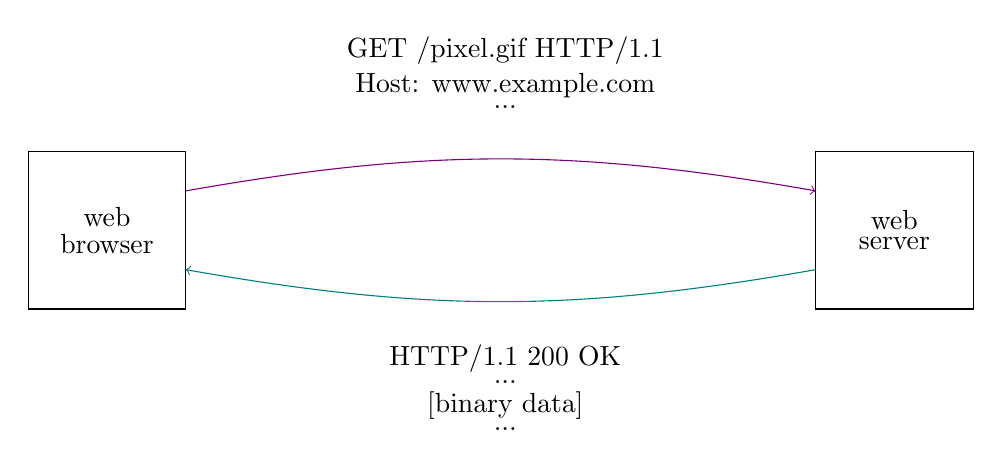
\begin{tikzpicture}
                        \node at (6, 1) {\shortstack{~GET /pixel.gif HTTP/1.1~\\~Host: www.example.com~\\~...~}};
                        \node at (6, -3) {\shortstack{~HTTP/1.1 200 OK~\\~...~\\~[binary data]~\\~...~}};
                        \node at (1, -1) {\shortstack{web\\browser}};
                        \node at (11, -1) {\shortstack{web\\server}};
                        \draw (0, 0) -- (2, 0) -- (2, -2) -- (0, -2) -- cycle;
                        \draw (10, 0) -- (12, 0) -- (12, -2) -- (10, -2) -- cycle;
                        \draw[violet] (2, -0.5) edge[->, bend left=10] (10, -0.5);
                        \draw[teal] (10, -1.5) edge[->, bend left=10] (2, -1.5);
                    \end{tikzpicture}
                \end{center}
            \subsubsection*{Layers}
                \begin{itemize}
                    \itemsep0em
                    \item \textbf{application layer}
                        \medskip

                        Any software written for the internet is on the application layer.
                    \item \textbf{transport layer}
                        \medskip

                        In the \textbf{transport layer}, packets leave your (client) machine to the server, and the server sends back packets to your client.
                        This layer divides a (big) message into smaller chunks, and sends them to the other side (re-ordered) to be presented to the recipient.
                    \item \textbf{network layer}
                        \medskip

                        The \textbf{route / path} (sequences of switches a packet goes through) each packet takes can be different from the others, and is often the most optimal route available.
                        This is done on the \textbf{network layer}, which routers are a part of.
                        \begin{center}
                            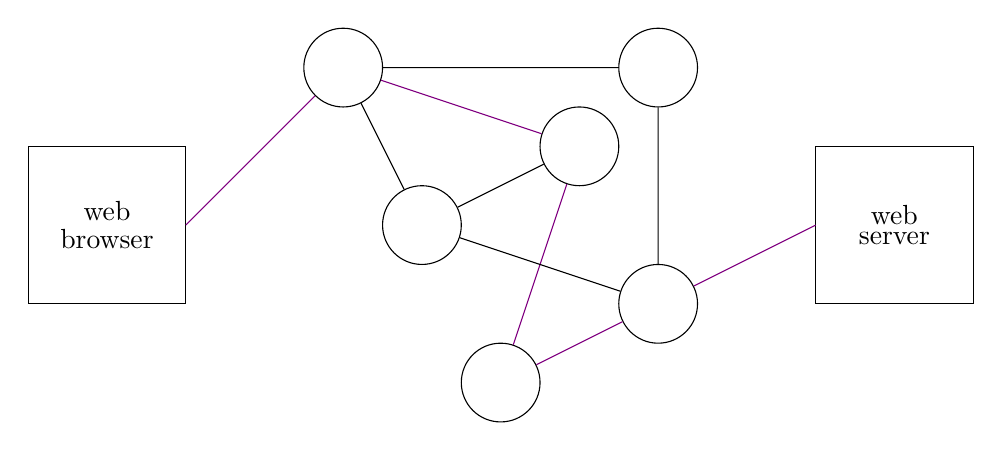
\begin{tikzpicture}
                                \node at (1, -1) {\shortstack{web\\browser}};
                                \node at (11, -1) {\shortstack{web\\server}};
                                \draw (0, 0) -- (2, 0) -- (2, -2) -- (0, -2) -- cycle;
                                \draw (10, 0) -- (12, 0) -- (12, -2) -- (10, -2) -- cycle;
                                \node[state, minimum size=1cm] (0) at (4, 1) {};
                                \node[state, minimum size=1cm] (1) at (5, -1) {};
                                \node[state, minimum size=1cm] (2) at (6, -3) {};
                                \node[state, minimum size=1cm] (3) at (7, 0) {};
                                \node[state, minimum size=1cm] (4) at (8, -2) {};
                                \node[state, minimum size=1cm] (5) at (8, 1) {};
                                \draw[violet] (2, -1) -- (0) -- (3) -- (2) -- (4) -- (10, -1);
                                \draw
                                (0) -- (1)
                                (0) -- (5)
                                (1) -- (3)
                                (1) -- (4)
                                (4) -- (5);
                            \end{tikzpicture}
                        \end{center}
                    \item \textbf{data link layer}
                        \medskip

                        Our devices are linked to the network on the \textbf{data link layer}, via network interface controllers (NICs).
                        Examples of this include Ethernet, fiber optic network cards, as well as wireless devices such as WiFi access points, and USB dongles for 4G.
                        A communication link is any connection between packet switches and / or end systems.
                    \item \textbf{physical layer}
                        \medskip

                        Finally, on the \textbf{physical layer}, there are various forms of communication media, including fiber-optic cables, twisted-pair copper wire, coaxial cables, and wireless local-area links (802.11, Bluetooth, etc).
                \end{itemize}
        \subsection*{16th January 2020 \hfill Week 2, Lecture 2}
            \subsubsection*{Circuit Switching}
                Old phones used circuit switching, which creates a connection between the two points, which is used for the entire communication.
                This isn't used for the internet as the failure of one node in the circuit would lead the the entire communication dropping - whereas a different route would be calculated in packet switching.
                \medskip

                Compared to packet switching, it has an expensive setup phase, but will need very little processing once the connection is established.
                However, it is inefficient for sharing resources - if a node is used as part of a circuit, it cannot be used by another connection for a different circuit.
                The resources are blocked once a connection is established (hence it is an inefficient way to use the network).
                On the other hand, packet switching has no setup cost, but has a processing cost, as well as space overhead, for every packet.
                It has a processing cost for forwarding the packets, as well as space overhead as there must be redundant data for each packet, such that it is self contained.
                It is specifically designed to share links, hence it allows for a better utilisation of network resources.
            \subsubsection*{Protocols}
                A protocol is a set of rules (an agreement between communicating parties on how communication is to proceed), run by end systems as well as packet switches.
                It must be unambiguous, complete (includes actions and / or responses for all possible situations), and also define all necessary message formats.
                The phases are as follows;
                \begin{itemize}
                    \itemsep0em
                    \item \textbf{handshake} \hfill establishes identities and / or context
                    \item \textbf{conversation} \hfill free-form exchange
                    \item \textbf{closing} \hfill terminating the conversation
                \end{itemize}
                The internet protocol stack is based on the 5 layers briefly covered in the previous lecture.
                Some examples of design issues that can be encountered are as follows;
                \begin{itemize}
                    \itemsep0em
                    \item \textbf{addressing} \hfill how to denote the intended recipient
                    \item \textbf{error control} \hfill how to detect (and possibly fix) transmission errors, e.g. checksums
                    \item \textbf{flow control} \hfill ensure data travels through communication media without issues
                    \item \textbf{multiplexing / demultiplexing} \hfill conversion of data into binary, and parallel communications
                    \item \textbf{routing} \hfill which route is chosen
                \end{itemize}
                Most network layers are either connection-oriented, where a connection is first established, data is exchanged, and the connection is finally released, or connectionless, where data is marked with its destination.
                \medskip

                The TCP/IP (4 layer) stack consists of application, transport, internet, and network access (which combines data link and physical).
                On the other hand, the OSI (7 layer) model consists of the application layer, presentation, session, transport, network, data link, and physical.
                \begin{center}
                    \hfill
                    \begin{tabular}{|c|}
                        \hline
                        \violet{application} \\
                        \hline
                        \violet{presentation} \\
                        \hline
                        \violet{session} \\
                        \hline
                        \blue{transport} \\
                        \hline
                        \red{network} \\
                        \hline
                        \teal{data link} \\
                        \hline
                        \teal{physical} \\
                        \hline
                    \end{tabular}
                    \hfill
                    \begin{tabular}{|c|}
                        \hline
                        \violet{application} \\
                        \hline
                        \blue{transport} \\
                        \hline
                        \red{network / internet} \\
                        \hline
                        \teal{data link} \\
                        \hline
                        \teal{physical} \\
                        \hline
                    \end{tabular}
                    \hfill
                    \begin{tabular}{|c|}
                        \hline
                        \violet{application} \\
                        \hline
                        \blue{transport} \\
                        \hline
                        \red{internet} \\
                        \hline
                        \teal{network access} \\
                        \hline
                    \end{tabular}
                    \hfill \phantom{}
                \end{center}
                A \textbf{service} is a set of primitives that a layer provides to the layer above it, whereas a \textbf{protocol} is a set of rules that prescribe the layout and meaning of packets.
                In a protocol stack, layer $k$ puts its entire packet as data into a layer $k - 1$ packet, the latter may add a header and / or a trailer.
                This may have to be split across several lower level packets (\textbf{fragmentation}).
                An example of protocol layering is as follows;
                \begin{center}
                    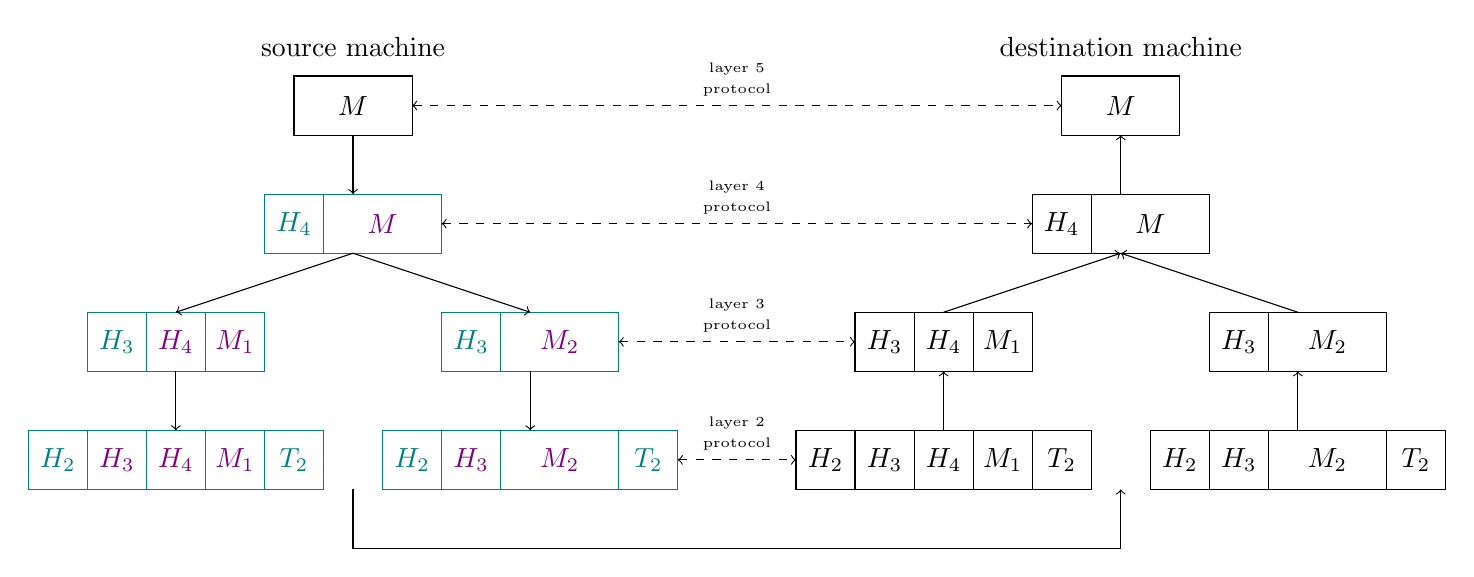
\begin{tikzpicture}[x=0.75cm, y=0.75cm]
                        \begin{scope}[shift={(0, 0)}]
                            \node at (1, 0.5) {source machine};
                            \node at (1, -0.5) {$M$};
                            \node at (0, -2.5) {\teal{$H_4$}};
                            \node at (1.5, -2.5) {\violet{$M$}};
                            \node at (-3, -4.5) {\teal{$H_3$}};
                            \node at (-2, -4.5) {\violet{$H_4$}};
                            \node at (-1, -4.5) {\violet{$M_1$}};
                            \node at (3, -4.5) {\teal{$H_3$}};
                            \node at (4.5, -4.5) {\violet{$M_2$}};
                            \node at (-4, -6.5) {\teal{$H_2$}};
                            \node at (-3, -6.5) {\violet{$H_3$}};
                            \node at (-2, -6.5) {\violet{$H_4$}};
                            \node at (-1, -6.5) {\violet{$M_1$}};
                            \node at (0, -6.5) {\teal{$T_2$}};
                            \node at (2, -6.5) {\teal{$H_2$}};
                            \node at (3, -6.5) {\violet{$H_3$}};
                            \node at (4.5, -6.5) {\violet{$M_2$}};
                            \node at (6, -6.5) {\teal{$T_2$}};
                            \draw (0, 0) -- (2, 0) -- (2, -1) -- (0, -1) -- cycle;
                            \draw[teal] (-0.5, -2) -- (2.5, -2) -- (2.5, -3) -- (-0.5, -3) -- cycle
                            (0.5, -2) -- (0.5, -3);
                            \draw[teal] (-3.5, -4) -- (-0.5, -4) -- (-0.5, -5) -- (-3.5, -5) -- cycle
                            (-2.5, -4) -- (-2.5, -5)
                            (-1.5, -4) -- (-1.5, -5);
                            \draw[teal] (2.5, -4) -- (5.5, -4) -- (5.5, -5) -- (2.5, -5) -- cycle
                            (3.5, -4) -- (3.5, -5);
                            \draw[teal] (-4.5, -6) -- (0.5, -6) -- (0.5, -7) -- (-4.5, -7) -- cycle
                            (-3.5, -6) -- (-3.5, -7)
                            (-2.5, -6) -- (-2.5, -7)
                            (-1.5, -6) -- (-1.5, -7)
                            (-0.5, -6) -- (-0.5, -7);
                            \draw[teal] (1.5, -6) -- (6.5, -6) -- (6.5, -7) -- (1.5, -7) -- cycle
                            (2.5, -6) -- (2.5, -7)
                            (3.5, -6) -- (3.5, -7)
                            (5.5, -6) -- (5.5, -7);
                            \draw
                            (1, -1) edge[->] (1, -2)
                            (1, -3) edge[->] (-2, -4)
                            (1, -3) edge[->] (4, -4)
                            (-2, -5) edge[->] (-2, -6)
                            (4, -5) edge[->] (4, -6);
                        \end{scope}
                        \draw[dashed]
                        (2, -0.5) edge[<->, above] node{\tiny\shortstack{layer 5\\protocol}} (13, -0.5)
                        (2.5, -2.5) edge[<->, above] node{\tiny\shortstack{layer 4\\protocol}} (12.5, -2.5)
                        (5.5, -4.5) edge[<->, above] node{\tiny\shortstack{layer 3\\protocol}} (9.5, -4.5)
                        (6.5, -6.5) edge[<->, above] node{\tiny\shortstack{layer 2\\protocol}} (8.5, -6.5);
                        \draw
                        (1, -7) -- (1, -8) -- (14, -8) edge[->] (14, -7);
                        \begin{scope}[shift={(13, 0)}]
                            \node at (1, 0.5) {destination machine};
                            \node at (1, -0.5) {$M$};
                            \node at (0, -2.5) {$H_4$};
                            \node at (1.5, -2.5) {$M$};
                            \node at (-3, -4.5) {$H_3$};
                            \node at (-2, -4.5) {$H_4$};
                            \node at (-1, -4.5) {$M_1$};
                            \node at (3, -4.5) {$H_3$};
                            \node at (4.5, -4.5) {$M_2$};
                            \node at (-4, -6.5) {$H_2$};
                            \node at (-3, -6.5) {$H_3$};
                            \node at (-2, -6.5) {$H_4$};
                            \node at (-1, -6.5) {$M_1$};
                            \node at (0, -6.5) {$T_2$};
                            \node at (2, -6.5) {$H_2$};
                            \node at (3, -6.5) {$H_3$};
                            \node at (4.5, -6.5) {$M_2$};
                            \node at (6, -6.5) {$T_2$};
                            \draw (0, 0) -- (2, 0) -- (2, -1) -- (0, -1) -- cycle;
                            \draw (-0.5, -2) -- (2.5, -2) -- (2.5, -3) -- (-0.5, -3) -- cycle
                            (0.5, -2) -- (0.5, -3);
                            \draw (-3.5, -4) -- (-0.5, -4) -- (-0.5, -5) -- (-3.5, -5) -- cycle
                            (-2.5, -4) -- (-2.5, -5)
                            (-1.5, -4) -- (-1.5, -5);
                            \draw (2.5, -4) -- (5.5, -4) -- (5.5, -5) -- (2.5, -5) -- cycle
                            (3.5, -4) -- (3.5, -5);
                            \draw (-4.5, -6) -- (0.5, -6) -- (0.5, -7) -- (-4.5, -7) -- cycle
                            (-3.5, -6) -- (-3.5, -7)
                            (-2.5, -6) -- (-2.5, -7)
                            (-1.5, -6) -- (-1.5, -7)
                            (-0.5, -6) -- (-0.5, -7);
                            \draw (1.5, -6) -- (6.5, -6) -- (6.5, -7) -- (1.5, -7) -- cycle
                            (2.5, -6) -- (2.5, -7)
                            (3.5, -6) -- (3.5, -7)
                            (5.5, -6) -- (5.5, -7);
                            \draw
                            (1, -1) edge[<-] (1, -2)
                            (1, -3) edge[<-] (-2, -4)
                            (1, -3) edge[<-] (4, -4)
                            (-2, -5) edge[<-] (-2, -6)
                            (4, -5) edge[<-] (4, -6);
                        \end{scope}
                    \end{tikzpicture}
                \end{center}
                Note that the connection between the two machines can have multiple nodes in between, that can read up to a different physical layer.
                For example, if there was a link-layer switch after the source machine, it can read up to the link layer (layer 2), remove and add headers / trailers, and then send it on to the next device.
                The next device may be a router for example, which can read up to the network layer (layer 3), and do the same.
                \medskip

                The data from the layer above is known as the \violet{SDU (service data unit)}, and the SDU combined with a header, added by the current layer, is known as the \teal{PDU (protocol data unit)}.
\end{document}